% Created by tikzDevice version 0.12.5 on 2024-01-22 14:46:46
% !TEX encoding = UTF-8 Unicode
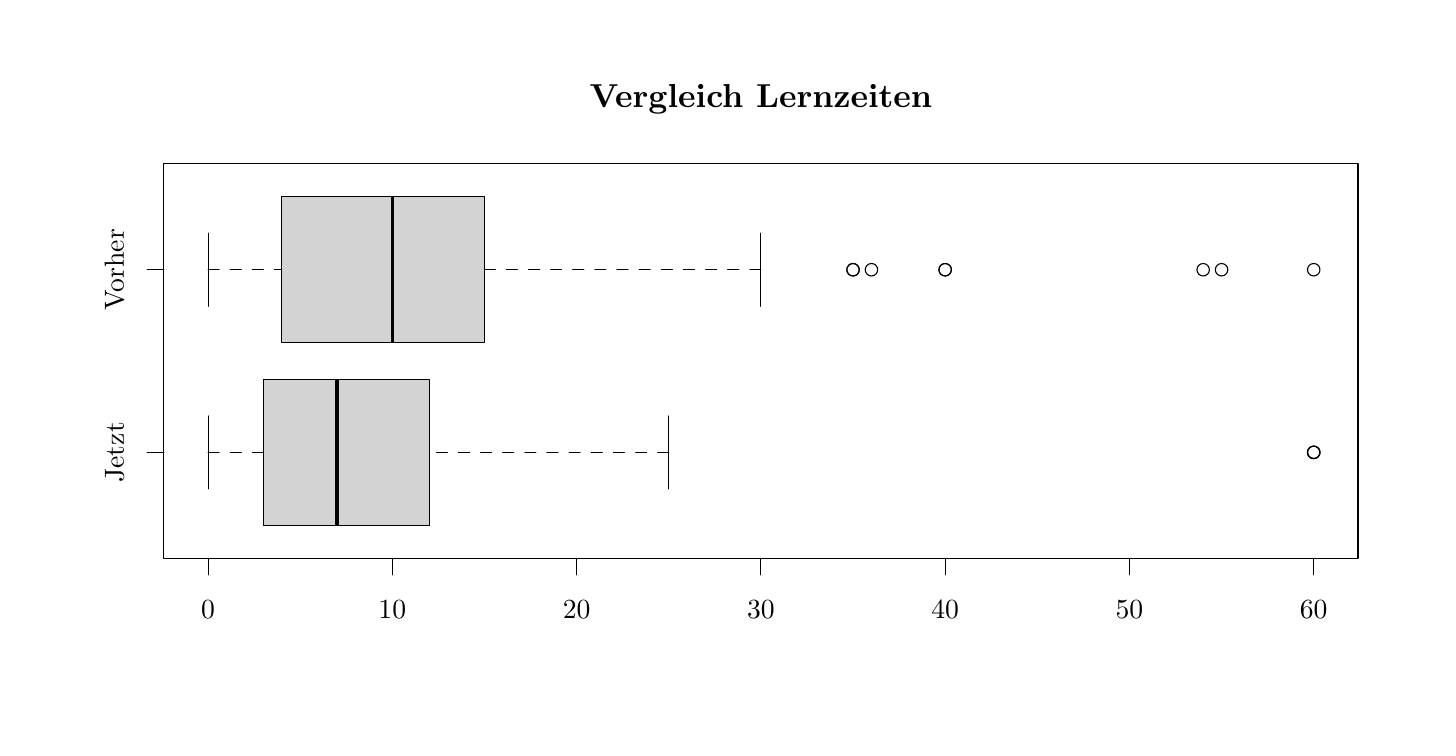
\begin{tikzpicture}[x=1pt,y=1pt]
\definecolor{fillColor}{RGB}{255,255,255}
\path[use as bounding box,fill=fillColor,fill opacity=0.00] (0,0) rectangle (505.89,252.94);
\begin{scope}
\path[clip] ( 49.20, 61.20) rectangle (480.69,203.75);
\definecolor{fillColor}{RGB}{211,211,211}

\path[fill=fillColor] ( 85.16, 73.08) --
	( 85.16,125.87) --
	(145.09,125.87) --
	(145.09, 73.08) --
	cycle;
\definecolor{drawColor}{RGB}{0,0,0}

\path[draw=drawColor,line width= 1.2pt,line join=round] (111.79, 73.08) -- (111.79,125.87);

\path[draw=drawColor,line width= 0.4pt,dash pattern=on 4pt off 4pt ,line join=round,line cap=round] ( 65.18, 99.48) -- ( 85.16, 99.48);

\path[draw=drawColor,line width= 0.4pt,dash pattern=on 4pt off 4pt ,line join=round,line cap=round] (231.65, 99.48) -- (145.09, 99.48);

\path[draw=drawColor,line width= 0.4pt,line join=round,line cap=round] ( 65.18, 86.28) -- ( 65.18,112.67);

\path[draw=drawColor,line width= 0.4pt,line join=round,line cap=round] (231.65, 86.28) -- (231.65,112.67);

\path[draw=drawColor,line width= 0.4pt,line join=round,line cap=round] ( 85.16, 73.08) --
	( 85.16,125.87) --
	(145.09,125.87) --
	(145.09, 73.08) --
	cycle;

\path[draw=drawColor,line width= 0.4pt,line join=round,line cap=round] (464.71, 99.48) circle (  2.25);

\path[draw=drawColor,line width= 0.4pt,line join=round,line cap=round] (464.71, 99.48) circle (  2.25);

\path[draw=drawColor,line width= 0.4pt,line join=round,line cap=round] (624.52, 99.48) circle (  2.25);

\path[draw=drawColor,line width= 0.4pt,line join=round,line cap=round] (464.71, 99.48) circle (  2.25);

\path[fill=fillColor] ( 91.82,139.07) --
	( 91.82,191.87) --
	(165.06,191.87) --
	(165.06,139.07) --
	cycle;

\path[draw=drawColor,line width= 1.2pt,line join=round] (131.77,139.07) -- (131.77,191.87);

\path[draw=drawColor,line width= 0.4pt,dash pattern=on 4pt off 4pt ,line join=round,line cap=round] ( 65.18,165.47) -- ( 91.82,165.47);

\path[draw=drawColor,line width= 0.4pt,dash pattern=on 4pt off 4pt ,line join=round,line cap=round] (264.95,165.47) -- (165.06,165.47);

\path[draw=drawColor,line width= 0.4pt,line join=round,line cap=round] ( 65.18,152.27) -- ( 65.18,178.67);

\path[draw=drawColor,line width= 0.4pt,line join=round,line cap=round] (264.95,152.27) -- (264.95,178.67);

\path[draw=drawColor,line width= 0.4pt,line join=round,line cap=round] ( 91.82,139.07) --
	( 91.82,191.87) --
	(165.06,191.87) --
	(165.06,139.07) --
	cycle;

\path[draw=drawColor,line width= 0.4pt,line join=round,line cap=round] (431.41,165.47) circle (  2.25);

\path[draw=drawColor,line width= 0.4pt,line join=round,line cap=round] (298.24,165.47) circle (  2.25);

\path[draw=drawColor,line width= 0.4pt,line join=round,line cap=round] (331.53,165.47) circle (  2.25);

\path[draw=drawColor,line width= 0.4pt,line join=round,line cap=round] (298.24,165.47) circle (  2.25);

\path[draw=drawColor,line width= 0.4pt,line join=round,line cap=round] (304.90,165.47) circle (  2.25);

\path[draw=drawColor,line width= 0.4pt,line join=round,line cap=round] (464.71,165.47) circle (  2.25);

\path[draw=drawColor,line width= 0.4pt,line join=round,line cap=round] (424.76,165.47) circle (  2.25);

\path[draw=drawColor,line width= 0.4pt,line join=round,line cap=round] (331.53,165.47) circle (  2.25);
\end{scope}
\begin{scope}
\path[clip] (  0.00,  0.00) rectangle (505.89,252.94);
\definecolor{drawColor}{RGB}{0,0,0}

\path[draw=drawColor,line width= 0.4pt,line join=round,line cap=round] ( 49.20, 99.48) -- ( 49.20,165.47);

\path[draw=drawColor,line width= 0.4pt,line join=round,line cap=round] ( 49.20, 99.48) -- ( 43.20, 99.48);

\path[draw=drawColor,line width= 0.4pt,line join=round,line cap=round] ( 49.20,165.47) -- ( 43.20,165.47);

\node[text=drawColor,rotate= 90.00,anchor=base,inner sep=0pt, outer sep=0pt, scale=  1.00] at ( 34.80, 99.48) {Jetzt};

\node[text=drawColor,rotate= 90.00,anchor=base,inner sep=0pt, outer sep=0pt, scale=  1.00] at ( 34.80,165.47) {Vorher};

\path[draw=drawColor,line width= 0.4pt,line join=round,line cap=round] ( 65.18, 61.20) -- (464.71, 61.20);

\path[draw=drawColor,line width= 0.4pt,line join=round,line cap=round] ( 65.18, 61.20) -- ( 65.18, 55.20);

\path[draw=drawColor,line width= 0.4pt,line join=round,line cap=round] (131.77, 61.20) -- (131.77, 55.20);

\path[draw=drawColor,line width= 0.4pt,line join=round,line cap=round] (198.36, 61.20) -- (198.36, 55.20);

\path[draw=drawColor,line width= 0.4pt,line join=round,line cap=round] (264.95, 61.20) -- (264.95, 55.20);

\path[draw=drawColor,line width= 0.4pt,line join=round,line cap=round] (331.53, 61.20) -- (331.53, 55.20);

\path[draw=drawColor,line width= 0.4pt,line join=round,line cap=round] (398.12, 61.20) -- (398.12, 55.20);

\path[draw=drawColor,line width= 0.4pt,line join=round,line cap=round] (464.71, 61.20) -- (464.71, 55.20);

\node[text=drawColor,anchor=base,inner sep=0pt, outer sep=0pt, scale=  1.00] at ( 65.18, 39.60) {0};

\node[text=drawColor,anchor=base,inner sep=0pt, outer sep=0pt, scale=  1.00] at (131.77, 39.60) {10};

\node[text=drawColor,anchor=base,inner sep=0pt, outer sep=0pt, scale=  1.00] at (198.36, 39.60) {20};

\node[text=drawColor,anchor=base,inner sep=0pt, outer sep=0pt, scale=  1.00] at (264.95, 39.60) {30};

\node[text=drawColor,anchor=base,inner sep=0pt, outer sep=0pt, scale=  1.00] at (331.53, 39.60) {40};

\node[text=drawColor,anchor=base,inner sep=0pt, outer sep=0pt, scale=  1.00] at (398.12, 39.60) {50};

\node[text=drawColor,anchor=base,inner sep=0pt, outer sep=0pt, scale=  1.00] at (464.71, 39.60) {60};
\end{scope}
\begin{scope}
\path[clip] (  0.00,  0.00) rectangle (505.89,252.94);
\definecolor{drawColor}{RGB}{0,0,0}

\node[text=drawColor,anchor=base,inner sep=0pt, outer sep=0pt, scale=  1.20] at (264.94,224.20) {\bfseries Vergleich Lernzeiten};
\end{scope}
\begin{scope}
\path[clip] (  0.00,  0.00) rectangle (505.89,252.94);
\definecolor{drawColor}{RGB}{0,0,0}

\path[draw=drawColor,line width= 0.4pt,line join=round,line cap=round] ( 49.20, 61.20) --
	(480.69, 61.20) --
	(480.69,203.75) --
	( 49.20,203.75) --
	cycle;
\end{scope}
\end{tikzpicture}
